\documentclass{beamer}
\usetheme{Madrid}
\usecolortheme{default}

\usepackage{amsmath, amssymb, amsfonts}
\usepackage{graphicx}
\usepackage{booktabs}

\newcommand{\eps}{\epsilon}

% --- Metadata ---
\title[FEM for Convection-Diffusion]{Finite Element Approximation of Convection-Diffusion Equation}
\subtitle{Vanishing Diffusion Limit and SUPG Stabilization}
\author{Devansh Tripathi}
\date{\today}

\begin{document}

% --- Slide 1: Title ---
\begin{frame}
    \titlepage
\end{frame}

% --- Slide 2: Abstract/Overview ---
\begin{frame}{Timeline of the talk}
    \begin{itemize}
        \item Model Problem: 1D steady-state convection-diffusion equation. \vspace{0.3cm}
        \item Weak formulation and standard Galerkin FEM.\vspace{0.3cm}
        \item Well-posedness \vspace{0.3cm}
        \item SUPG stabilization method and its well-posedness.\vspace{0.3cm}
        \item Error analysis of SUPG. \vspace{0.3cm}
        \item Test Problem: 1D boundary layer. \vspace{0.3cm}
        \item Numerical results comparing Galerkin and SUPG. \vspace{0.3cm}
        \item Conclusion and future work. \vspace{0.3cm}
    \end{itemize}
\end{frame}

% --- Slide 3: Problem Statement ---
\begin{frame}{Model Problem}
    Consider the steady-state 1D convection-diffusion equation:
    \begin{equation}
        -\epsilon \Delta u(x) + \mathbf{b}\cdot \nabla u(x) = f(x), \quad x \in (0,1)
    \end{equation}
    with Dirichlet boundary conditions:
    \begin{equation}
        u(0) = 0, \quad u(1) = 0
    \end{equation}
    \begin{itemize}
        \item $\epsilon$: Diffusion coefficient ($0 < \epsilon < 1$)
        \item $\textbf{b}$: convection field.
        \item $f \in L^2(0,1).$
    \end{itemize}
\end{frame}

% --- Slide 4: Weak Formulation ---
\begin{frame}{Weak Formulation}
    Find $u \in V = H_0^1(0,1)$ such that $a(u,v) = l(v) \quad \forall v \in V$.
    \vfill
    \textbf{Bilinear Form:}
    \begin{equation*}
        a(u,v) = \epsilon (\nabla u, \nabla v) + (\textbf{b} \cdot \nabla u, v)
    \end{equation*}
    \textbf{Linear Functional:}
    \begin{equation*}
        l(v) = (f, v)
    \end{equation*}
    \pause
    \textbf{Discrete space:}
    \begin{equation*}
        V_h = \{ v_h \in C[0, 1] \mid v_h|_{I_i} = P_1(I_i) \ \forall i, \ v_h(0) = 0 = v_h(1)\} \subset V.
    \end{equation*}
\end{frame}


% --- Slide 5: Well-posedness & Galerkin Failure ---
\begin{frame}{Well-posedneses: Lax-Milgram}
    Well-posedness is guaranteed if $a(\cdot,\cdot)$ is bounded and coercive.
    \begin{itemize}
        \item For coercivity: $a(v,v) = \epsilon ||\nabla v||^2_{L^2}$.
        \item Using Poincaré inequality, we find $a(v,v) \ge \alpha \|v\|_{L^2(0,1)}^2$ where $\alpha = \frac{\epsilon}{C^2}$.
    \end{itemize}
    \vfill
    \pause
    \textbf{Critical Failure as $\epsilon \to 0$:}
    \begin{itemize}
        \item The coercivity constant $\alpha$ is directly proportional to $\epsilon$.
        \item As $\epsilon \to 0$, the bilinear form loses its coercive property.
        \item Stability estimate $||u||_V \le \frac{1}{\alpha} ||f||_{L^2}$ ``blow up" leading to massive spurious oscillations.
    \end{itemize}
\end{frame}

% --- Slide 6: SUPG Stabilization ---
\begin{frame}{SUPG: Streamline-Upwind Petrov-Galerkin}
    SUPG adds artificial diffusion \textbf{only} in the streamline direction to provide stability.
    \vfill
    \pause
    Discrete space changes: $u_h$ has to be $H^2$-conforming to compute the strong residual $R(u_h)$ inside each element.
    \vfill
    \pause
    \textbf{Stabilized Formulation:}
    \begin{equation}
        a_h(u_h,v_h) + \sum_{i} (R(u_h), \tau_i \textbf{b} \cdot \nabla v_h)_{I_i} = (f, v_h)
    \end{equation}
    where $R(u_h) = -\epsilon \Delta u_h + \textbf{b} \cdot \nabla u_h - f$ is the strong residual.
    \begin{itemize}
        \item $\tau$ is the stabilization parameter tuned to the P\'eclet number.
        \item SUPG is \textbf{consistent}: the exact solution $u$ satisfies the equation since $R(u)=0$.
    \end{itemize}
\end{frame}

% --- Slide 8: Well-posedness of SUPG
\begin{frame}{Well-Posedness of SUPG}
\textbf{Streamline-Diffusion norm:}
\begin{equation}
    \boxed{|||v|||_{SD} := \left(\eps \| \nabla v\|^2_{L^2(0,1)} + \sum_{I_i} \tau_{i} \|\textbf{b} \cdot \nabla v\|^2_{L^2(I_i)} + \omega \|v\|^2_{L^2(I_i)}\right)^{1/2}}
\end{equation}
\vfill
\pause
For stability of the SDFEM, let the constant $\omega$ satisfy 
$$ c-\frac{1}{2} \nabla \cdot b \geq \omega > 0 \text{  on  } \Omega = (0,1).$$
\pause
We can not have divergence-free field and reaction coefficient to be 0 simultaneously. Atleast, this analysis will fail!!!
\end{frame}

\begin{frame}{Local Inverse Inequality}
% \kern-0.4em
\begin{lemma}[Local Inverse Inequality]
    For the discrete finite element space $V_h$, there exists a constant $\mu_{\text{inv}} > 0$, independent of the element $I_i$ and the local mesh size $h_{I_i}$, such that
    \begin{equation*}
        \|\Delta v_h\|_{L^2(I_i)} \leq \mu_{\text{inv}} h_{I_i}^{-1} |v_h|_{H^1(I_i)} \quad \forall v_h \in V_h
    \end{equation*}
\end{lemma}
\pause
\begin{lemma}\label{lem:sdparam}
    Let the SD parameter $\tau_i$ satisfy
    $$ 0 < \tau_i \leq \frac{1}{2} \frac{h_{I_i}^2}{\eps\mu_{inv}^2}$$
    for each $i$ where $I_i$ is the $i^{th}$ element. Then the bilinear form is coercive, i.e.
    $$a_h(v_h, v_h) \geq \frac{1}{2} ||| v_h|||^2_{SD} \qquad \forall v_h \in V_h.$$
\end{lemma}
% \kern-0.7em
% \pause

\end{frame}

\begin{frame}{Stability estimate: SUPG}
\kern-0.6em
\begin{proof}
\kern-1.2em
     \begin{align*}
        a_{SUPG}(v_h, v_h) = \epsilon \|\nabla v_h\|^2_{L^2} + (\textbf{b} \cdot \nabla v_h, v_h) &- \sum_{i} \tau_i (\eps\Delta v_h, \textbf{b} \cdot \nabla v_h)_{I_i}  \\ &+ \sum_{i} \tau_i \|\textbf{b} \cdot \nabla v_h\|_{I_i}^2
    \end{align*}
\end{proof}
\pause
Stability estimate:
$$ \boxed{|||u|||_{SD} \leq C\left( \|f\|_{L^2(0,1)}^2 + \sum_{I_i} \tau_i \|f\|^2_{L^2(I_i)}\right)^{1/2}}$$
$C$ is independent of $\eps$.
\pause
\begin{proof}
    Cauchy-Schwartz and $\|u\|_{L^2} \leq C|||u|||_{SD}$.
\end{proof}
    
\end{frame}

\begin{frame}{Error Analysis: SUPG}
\begin{theorem}[1]
    Let the hypotheses of Lemma \ref{lem:sdparam} be satisfied. Choose $\tau_i$ such that
    $$\tau_i = \begin{cases}
        \delta_0 h_{I_i} \qquad \quad Pe_{I_i} > 1 \qquad \text{convection-dominated case,} \\
        \delta_1 h_{I_i}^2/\eps \qquad Pe_{I_i} \leq 1 \qquad \text{diffusion-dominated case,}
    \end{cases}$$
    with appropriate positive constants $\delta_0$ and $\delta_1$. Then the solution $u_h$ of the SDFEM satisfies the global error estimate
    $$ |||u - u_h|||_{SD} \leq C(\eps^{1/2} + h^{1/2})h^k |u|_{H^{k+1}}.$$
\end{theorem}
The \textit{local mesh P\'eclet number} is defined as:
$$Pe_{I_i} := \frac{\|b\|_{L^\infty(I_i)} h_{I_i}}{2\epsilon} = \frac{\text{Advection Rate}}{\text{Diffusion Rate}}$$
    
\end{frame}

% --- Slide 7: The Boundary Layer Problem ---
\begin{frame}{The Diffusion Limit $\epsilon \to 0$}
    \begin{itemize}
        \item When $\epsilon \to 0$, the equation becomes $\textbf{b} \cdot \nabla u = f$, a 1st-order hyperbolic PDE. \pause
        \item This requires only one boundary condition. \pause
        \item To satisfy both $u(0)=0$ and $u(1)=c \neq 0$, the solution must change abruptly near the boundary. \pause
        \item Standard Galerkin (central difference-like) cannot resolve this without $h \sim O(\epsilon)$.
    \end{itemize}
    \vspace{0.1em}
    \pause
    \textbf{Problem:} \textit{1D Boundary Layer}
    \begin{align*}
    -\varepsilon u''(x) + \,u'(x) &= 0, \quad x \in (0,1), \\
    u(0) &= 0, \\
    u(1) &= 1.
    \end{align*}
    \pause
    \textbf{Exact solution:}
    \vspace{-0.25em}
    \begin{align*}
    u(x) = \frac{e^{\frac{x-1}{\varepsilon}} - e^{-\frac{1}{\varepsilon}}}{1 - e^{-\frac{1}{\varepsilon}}}.
    \end{align*}
\end{frame}

% --- Slide 8: Numerical Results (Test 1) ---
\begin{frame}{Test 1: 1D Boundary Layer — Galerkin}
\centering
\vspace{-0.15cm}
% -------- TOP ROW --------
\begin{minipage}{0.48\textwidth}
\centering
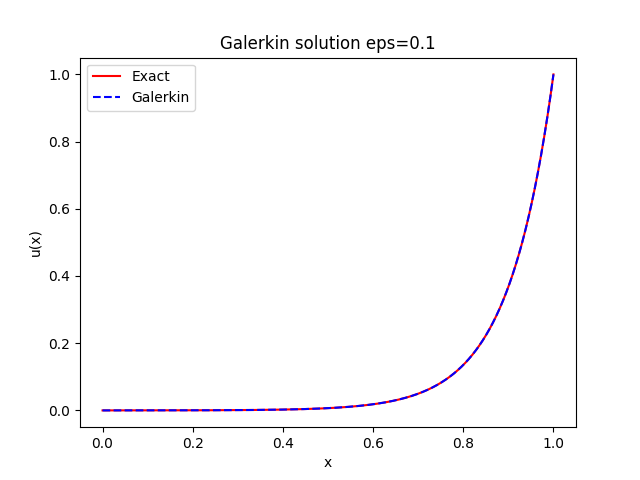
\includegraphics[width=\linewidth]{galerkin_eps_0.1.png}
\vspace{0.2cm}
\pause
% $\varepsilon = 10^{-1}$
\end{minipage}
\hfill
\begin{minipage}{0.48\textwidth}
\centering
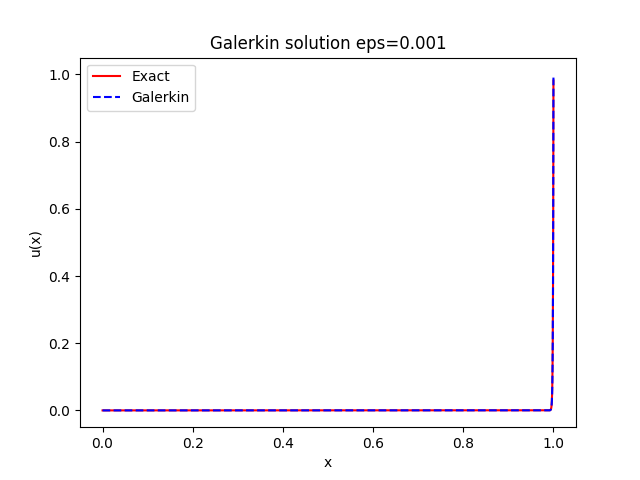
\includegraphics[width=\linewidth]{galerkin_eps_0.001.png}
\vspace{0.2cm}
\pause
% $\varepsilon = 10^{-3}$
\end{minipage}

\vspace{-1.1cm}

% -------- BOTTOM ROW --------
\begin{minipage}{0.5\textwidth}
\centering
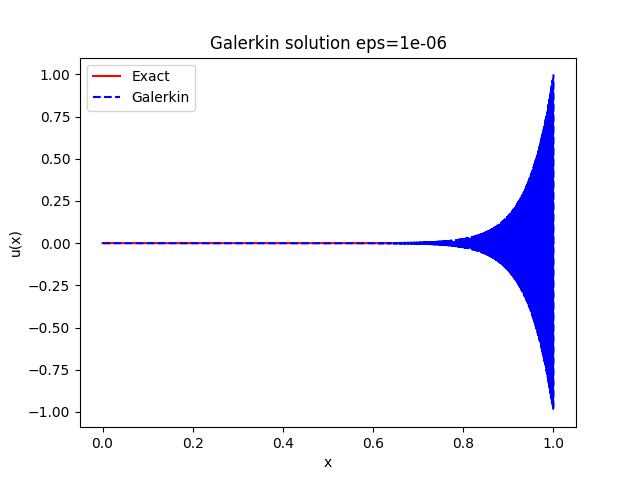
\includegraphics[width=\linewidth]{galerkin_eps_1e-06.png}
\vspace{0.2cm}

% $\varepsilon = 10^{-6}$
\end{minipage}

% \vspace{0.3cm}
% {\large Galerkin}

\end{frame}
\begin{frame}{Test 1: 1D Boundary Layer — SUPG}
\centering
\vspace{-0.15cm}
    % -------- TOP ROW --------
\begin{minipage}{0.48\textwidth}
\centering
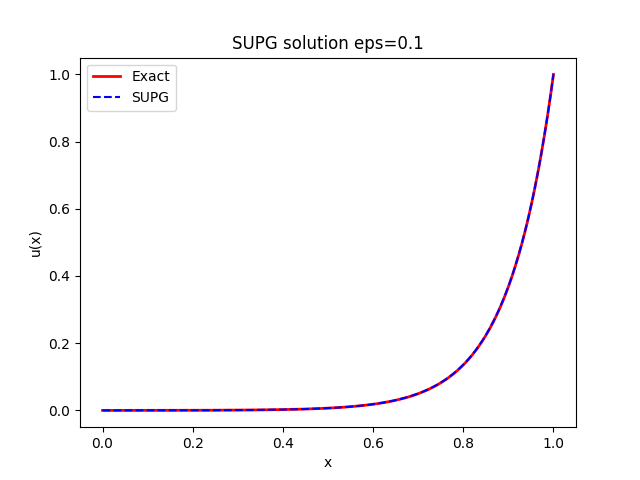
\includegraphics[width=\linewidth]{SUPG_eps_0.1.png}
\vspace{0.2cm}
\pause
% $\varepsilon = 10^{-1}$
\end{minipage}
\hfill
\begin{minipage}{0.48\textwidth}
\centering
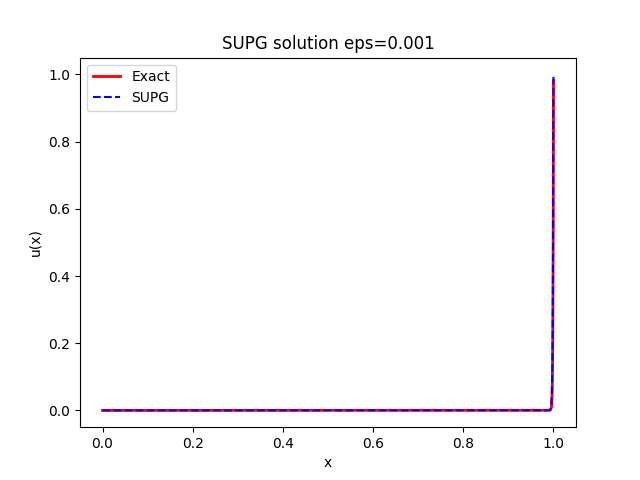
\includegraphics[width=\linewidth]{SUPG_eps_0.001.png}
\vspace{0.2cm}
\pause
% $\varepsilon = 10^{-3}$
\end{minipage}

\vspace{-1cm}

% -------- BOTTOM ROW --------
\begin{minipage}{0.5\textwidth}
\centering
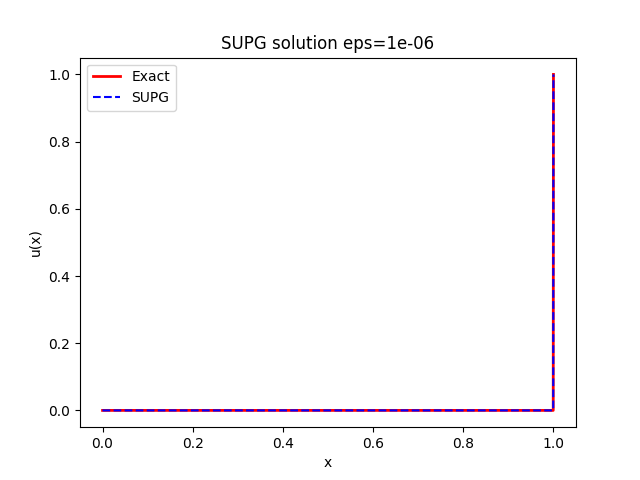
\includegraphics[width=\linewidth]{SUPG_eps_1e-06.png}
\vspace{0.2cm}

% $\varepsilon = 10^{-6}$
\end{minipage}

% \vspace{0.3cm}
% {\large SUPG}

\end{frame}

% --- Slide 9: Numerical Data ---
\begin{frame}{Error Comparison ($h=0.0005$)}
    \centering
    \begin{table}
        \begin{tabular}{l l l l}
            \toprule
            $\epsilon$ & Method & $||u-u_h||_{L^2}$ & $|u-u_h|_{H^1}$ \\
            \midrule
            $10^{-1}$ & Galerkin & 3.29e-7 & 7.35e-6 \\
            $10^{-3}$ & Galerkin & 3.24e-4 & 6.2e-1 \\
            $10^{-6}$ & Galerkin & 0.1020 & 707.106 \\
            \midrule \pause
            $10^{-1}$ & SUPG & 0.0003 & 0.0039 \\
            $10^{-3}$ & SUPG & 3.75e-3 & 2.80 \\
            $10^{-6}$ & SUPG & 0.0129 & 44.632 \\
            \bottomrule
        \end{tabular}
    \end{table}
    Error in $H^1$ norm blows up significantly as $\epsilon$ decreases.
\end{frame}

% --- Slide 10: INTERNAL BOUNDARY LAYER (Placeholder) ---
% \begin{frame}{Test 2: Internal Boundary Layer}
%     \begin{itemize}
%         \item \textbf{Setup:} Discontinuous source or varying convection field.
%         \item \textbf{Plots:}
%             \vspace{2cm} % Space for your plot
%         \item \textbf{Analysis:}
%             \begin{itemize}
%                 \item Observe how SUPG handles internal transitions compared to Galerkin.
%             \end{itemize}
%     \end{itemize}
% \end{frame}

% --- Slide 11: Conclusion & Future Work ---
\begin{frame}{Conclusion}
    \begin{itemize}
        \item Galerkin FEM fails in convection-dominated regimes because coercivity constant $\alpha \to 0$. \pause
        \item Stability estimates blow up as $\epsilon \to 0$, leading to spurious oscillations. \pause
        \item SUPG provides a consistent way to add numerical diffusion. \pause
        \item Stabilization is essential for robust simulations in the vanishing diffusion limit. \pause
    \end{itemize}
    \vfill
    \textbf{Future Work:}
    \begin{itemize}
        \item Adaptive mesh refinement (Shishkin-type meshes).
        \item Comparison with Discontinuous Galerkin (DG) methods.
    \end{itemize}

\end{frame}
\begin{frame}{References}
    \begin{itemize}
        \item H.-G. Roos, M. Stynes, and L. Tobiska,\textit{Robust Numerical Methods for Singularly Perturbed Differential Equations: Convection-Diffusion -Reaction and Flow Problems}, 2nd ed., Springer, 2008.
        \vfill
        \item A. N. Brooks and T. J. R. Hughes, \textit{Streamline Upwind/Petrov -Galerkin formulations for convection dominated flows with particular emphasis on the incompressible Navier-Stokes equations}, Comput. Methods Appl. Mech. Engrg., 32 (1982), pp. 199--259.
    \end{itemize}
    \centering \vfill
    \textbf{Thank you!}
\end{frame}

\end{document}